\section{Auswertung}
\label{sec:Auswertung}

Für die Berechnung vieler Ergebnisse wird der Wert $U_0$ benötigt. Dieser wird auf einen Wert von \SI{621}{\milli\volt} gesetzt, damit die Rechnungen funktionieren. %\ref{sec: dis}
Bei der Auswertung bzw. Berechnung wird Python, im Speziellen matplotlib.pyplot \cite{matplotlib}, numpy \cite{numpy}, uncertainties.unumpy \cite{uncertainties} und scipy \cite{scipy} verwendet.

\subsection{Bestimmung von RC über den Entladevorgang des Kondensators}
\label{sec: a}
Die Zeitkonstante wird anhand der Steigung einer linearen Regression bestimmt.
Dazu wird die Gleichung für die Entladung eines Kondensators in die Form $y=mx+b$ gebracht:
\begin{equation}
    - \log(\frac{U(t)}{U_{0}}) = \frac{1}{RC} t.
    \label{eqn: linreg1}
\end{equation}
Der negative logarithmierte Quotient der Kondensatorspannung durch die maximale Spannung wird gegen die Zeit aufgetragen.
Die Steigung bei der linearen Regression ist gegeben durch
\begin{equation*}
    m = \frac{\overline{xy} - \overline{x}\overline{y}}{\overline{x^2} - \overline{x}^2}.
\end{equation*}
Die Steigung, wie aus Gleichung \eqref{eqn: linreg1} entnommen werden kann, wird durch
\begin{equation*}
    m = \frac{1}{RC}
\end{equation*}
beschrieben. Also wird $\frac{1}{RC}$ bestimmt durch
\begin{equation}
    \frac{1}{RC}= \frac{\overline{xy} - \overline{x}\overline{y}}{\overline{x^2} - \overline{x}^2}.
    \label{eqn: RC}
\end{equation}
Dabei sind, ebenfalls aus Gleichung \eqref{eqn: linreg1} entnehmbar, $x=t$ und $y=-\log(\frac{U(t)}{U_{0}})$. %nebeneinander schreiben?
Der Fehler der inversen Zeitkonstante ist gegeben durch
\begin{equation}
    \frac{1}{N} \sum_{i=1}^N f(x_{i}) - y_{i},
    \label{eqn: fehler}
\end{equation}
wobei $N$ die Anzahl der Datenpaare, 
$f(x_{i})$ die Werte des Fits an der Stelle $x_{i}$
und $y_{i}$ die gemessenen $y$-Werte an der Stelle $x_{i}$ sind.
Der Fehler gilt ebenfalls für die im Folgenden beschriebenen Zeitkonstanten.
\newline
Die Werte, die für die Bestimmung der Zeitkonstanten $RC$ nötig sind, befinden sich in Tabelle \ref{tab1}.
\begin{table}\caption{Die Länge der Zylinder und die Spannung mit den jeweiligen Zeitenpunkten der Ausschläge.}
\label{taba}
\centering
\sisetup{round-mode = places, round-precision=2, round-integer-to-decimal=true}
\begin{tabular}{S[]S[]S[]S[]S[]} 
\toprule
{$l/ \si{\milli\meter}$} & {$U_1/ \si{\volt}$} & {$t_1/ \si{\micro\second}$} & {$U_2/ \si{\volt}$} & {$t_2/ \si{\micro\second}$}\\
\midrule
120.8 & 1.29 & 0.6 & 0.17 & 88.7\\
102.3 & 1.27 & 0.5 & 0.2 & 76.5\\
80.5 & 1.33 & 0.6 & 0.76 & 59.8\\
40.4 & 1.33 & 0.5 & 1.34 & 30.2\\
31.1 & 1.29 & 0.5 & 1.37 & 23.8\\
\bottomrule
\end{tabular}\end{table}
Die $x$ und $y$ Werte der linearen Regression \eqref{eqn: linreg1} sind in Tabelle \ref{taba} dargestellt.
Abbildung \ref{fig:plota} stellt die Gerade dieser linearen Regression dar.
\begin{table}\caption{Der zeitliche Verlauf $t$ gegen den negativen Logarithmus der Spannungswerte geteilt durch die maximale Spannung}
\label{taba}
\centering
\sisetup{round-mode = places, round-precision=5, round-integer-to-decimal=true}
\begin{tabular}{S[]S[]} 
\toprule
{$t/ \si{\second}$} & {$-log(\frac{U(t)}{U_{0}})$}\\
\midrule
0.0 & -0.0\\
0.0004 & 0.13372577497521726\\
0.0008 & 0.4281699018019215\\
0.0012 & 0.705467664947986\\
0.0016 & 0.9977516783331359\\
0.003 & 1.3015531326648002\\
0.0024 & 1.623136756792262\\
0.0028 & 1.8993901334204206\\
0.0032 & 2.2178438645389553\\
0.0036 & 2.505525936990737\\
0.004 & 2.793208009442516\\
0.0044 & 3.19867311755068\\
0.0048 & 3.604138225658845\\
0.0052 & 4.29728540621879\\
0.0056 & 4.990432586778735\\
\bottomrule
\end{tabular}\end{table}

\begin{figure}
  \centering
  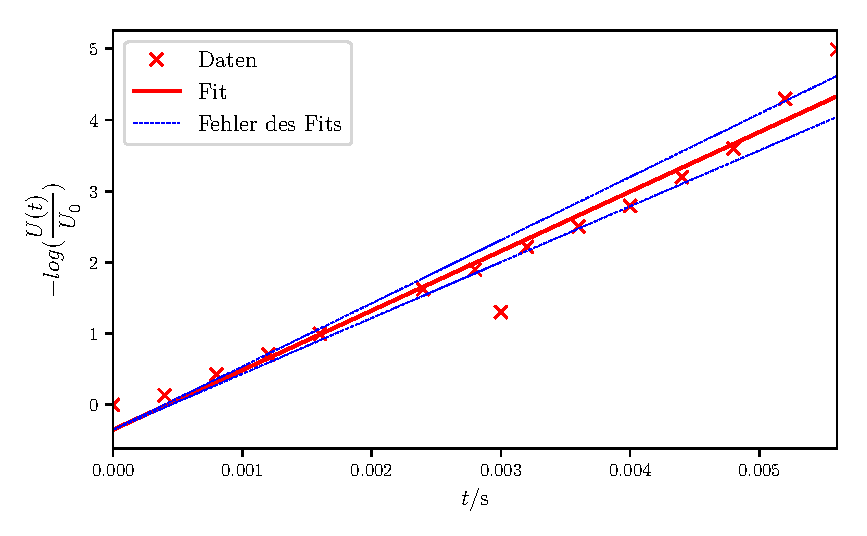
\includegraphics[width=13cm, height=9cm]{build/plota.pdf}
  \caption{Auftragung des negativen Logarithmus der Kondensatorpannung geteilt durch die maximale Spannung gegen die Zeit beim Entladevorgang.
  Dargestellt werden die Daten, der dazugehörige Fit und der Fehler des Fits.}
  \label{fig:plota}
\end{figure}

\noindent Die Steigung der Geraden ist das Inverse der Zeitkonstante.
Mittels Gleichung \eqref{eqn: RC} und der Gleichung für den Fehler \eqref{eqn: fehler} berechnet
sich das Inverse der Zeitkonstante zu $\frac{1}{RC} = \SI[per-mode=fraction]{836.500 \pm 51.514}{\per\second}$.

\subsection{Bestimmung von RC über die Amplitude der Kondensatorspannung}
\label{sec: b}
Um die Zeitkonstante $RC$ anhand der Amplitude der Kondensatorspannung zu bestimmen, wird wieder eine lineare Regression $y=mx+b$ durchgeführt. %Formulierung ändern
Die Gleichung \eqref{eqn: A2} wird so umgeformt, dass $\frac{1}{RC}$ die Steigung $m$ ist:
\begin{equation}
    \sqrt{\frac{1}{(\frac{U_{0}}{A(\omega)}})^2 -1} = \frac{1}{RC} \frac{1}{\omega}.
    \label{eqn: linreg2}
\end{equation}
Für x und y ergeben sich also: $x=\frac{1}{\omega}$ und $y=\sqrt{\frac{1}{(\frac{U_{0}}{A(\omega)}})^2 -1}$. %Doppelpunkt?
Durch die Steigung der Geraden kann dann $\frac{1}{RC}$ mittels \eqref{eqn: RC} bestimmt werden.
\newline
Die Kondensatorspannungen und die zeitlichen Phasenverschiebungen in Abhängigkeit
von der Frequenz sind in Tabelle \ref{tab2} dargstellt.
\begin{table}\caption{Die angelegte Spannung des elektrischen Feldes innerhalb des Geiger-Müller-Zählrohrs, die Anzahl der jeweils gemessenen Impulse und der Strom innerhalb des Geiger-Müller-Zählrohrs.}
\label{tabb}
\centering
\sisetup{round-mode = places, round-precision=2, round-integer-to-decimal=true}
\begin{tabular}{c c S[]} 
\toprule
{$U / \si{\volt}$} & {$\frac{N}{\SI{130}{\second}}$} & {$I / \si{\ampere}$}\\
\midrule
320 & 11298 & 0.1\\
400 & 11820 & 0.2\\
480 & 12135 & 0.3\\
540 & 12301 & 0.35\\
560 & 12068 & 0.4\\
600 & 12354 & 0.45\\
640 & 12403 & 0.5\\
660 & 12507 & 0.55\\
680 & 12659 & 0.6\\
\bottomrule
\end{tabular}\end{table}
Um die Zeitkonstante aus der Amplitude der Kondensatorspannung errechnen zu können, wird eine lineare Regression 
\eqref{eqn: linreg2} durchgeführt. Die $x$ und $y$ Werte dazu finden sich in Tabelle \ref{tabb}.
In Abbildung \ref{fig:plotb} sind diese $x$ und $y$ Werte gegeneinander aufgetragen.
\begin{table}\caption{}
\label{}
\centering
\sisetup{round-mode = places, round-precision=2, round-integer-to-decimal=true}
\begin{tabular}{S[]S[]} 
\toprule
{$\frac{1}{\omega}/ \si{\second}$} & {$\sqrt{\frac{1}{\frac{U_{0}}{A(\omega)}^{2}-1}}$}\\
\midrule
0.0024485375860291594 & 2.262660907951623\\
0.0019894367886486917 & 1.7091833258800144\\
0.0015915494309189533 & 1.2706566931710195\\
0.0006366197723675814 & 0.48280454958526764\\
0.00039788735772973834 & 0.2991883988251616\\
0.0002448537586029159 & 0.18505403427568887\\
0.00019894367886486917 & 0.14980117725462763\\
0.00015915494309189535 & 0.14980117725462763\\
6.366197723675813e-05 & 0.0483656490240811\\
3.978873577297384e-05 & 0.030287634503871775\\
2.448537586029159e-05 & 0.01884392449684891\\
1.989436788648692e-05 & 0.015621873649013022\\
1.5915494309189534e-05 & 0.01240030915098555\\
\bottomrule
\end{tabular}\end{table}

\begin{figure}
  \centering
  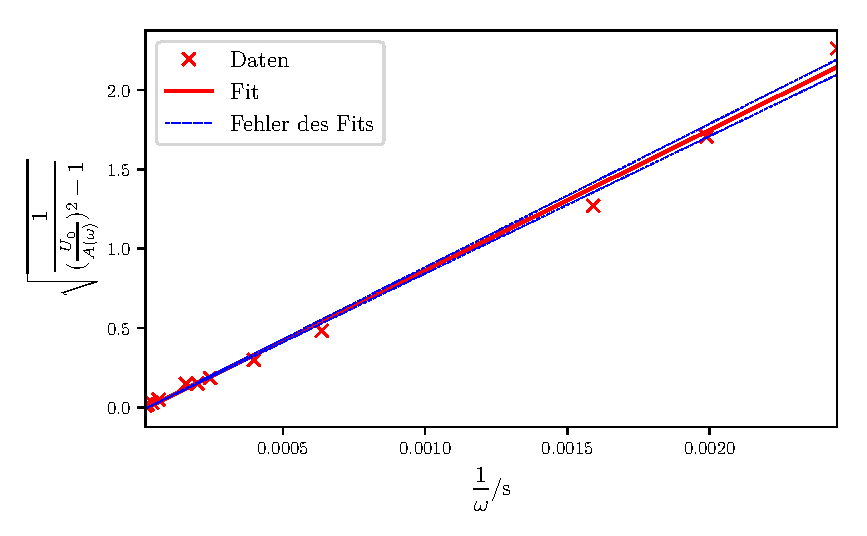
\includegraphics[width=13cm, height=9cm]{build/plotb.pdf}
  \caption{Auftragung der Wurzel aus dem Bruch in dessen Nenner die maximale Spannung durch die Amplitudenwerte von 
  $U_{C}$ zum Quadrat um eins subtrahiert werden gegen den Kehrwert der Kreisfrequenz. Dargestellt werden die Daten 
  und der zugehörige Fit. Die Skala ist logarithmiert.}
  \label{fig:plotb}
\end{figure}

\noindent Das Inverse der Zeitkonstante wird wieder durch \eqref{eqn: RC} und der Fehler durch \eqref{eqn: fehler}
berechnet. Es ergibt sich $\frac{1}{RC} = \SI[per-mode=fraction]{885.682  \pm 19.461}{\per\second}$.

\subsection{Bestimmung von RC über die Phasenverschiebung der Kondensatorspannung}
\label{sec: c}
Um die Zeitkonstante zu berechnen, wird wieder eine lineare Regression benötigt.
Die Gleichung \eqref{eqn: phi} wird so umgestellt, dass die Steigung $m = \frac{1}{RC}$ ist:
\begin{equation}
    -\frac{1}{\mathbf{tan}(\phi(\omega))} = \frac{1}{RC} \frac{1}{\omega}.
    \label{eqn: linreg3} 
\end{equation}
Dann ist $x= \frac{1}{\omega}$ und $y= -\frac{1}{\mathbf{tan}(\phi(\omega))}$.
$RC$ kann somit wieder durch \eqref{eqn: RC} bestimmt werden.
\newline
Die Abstände der Nulldurchgänge der Spannung des Kondensators und der Spannung des Generators in Abhängigkeit
von der Frequenz sind bereits in Tabelle \ref{tab2} aufgelistet.
Um die Zeitkonstante aus dieser Phasenverschiebung zu bestimmen, wird die lineare Regression \eqref{eqn: linreg3} benötigt.
Die $x$ und $y$ Werte befinden sich in Tabelle \ref{tabc}. Abbildung \ref{fig:plotc} stellt die Gerade der
linearen Regression dar, deren Steigung das Inverse der Zeitkonstante ist.
\begin{table}\caption{Der Kehrwert der Kreisfrequenz gegen den negativen Kehrwert des Tangens der Phase, die sich durch die negative Division der zeitlichen Phasenverschiebung durch die Periodendauer multipliziert mit \pi ergibt}
\label{tabc}
\centering
\sisetup{round-mode = places, round-precision=5, round-integer-to-decimal=true}
\begin{tabular}{S[]S[]} 
\toprule
{$\frac{1}{\omega}/ \si{\second}$} & {$-\frac{1}{tan(\phi(\omega))}$}\\
\midrule
0.0024485375860291594 & 3.117626187195526\\
0.0019894367886486917 & 2.723786837133246\\
0.0015915494309189533 & 2.2715973027329865\\
0.0006366197723675814 & 1.4714553158199692\\
0.00039788735772973834 & 1.2401991640705359\\
0.0002448537586029159 & 1.2010895549922853\\
0.00019894367886486917 & 1.120011792429241\\
0.00015915494309189535 & 1.0000000000000002\\
6.366197723675813e-05 & 0.8540806854634666\\
3.978873577297384e-05 & 1.0126459941540735\\
2.448537586029159e-05 & 1.0190294678742615\\
1.989436788648692e-05 & 1.064891840324792\\
1.5915494309189534e-05 & 1.064891840324792\\
\bottomrule
\end{tabular}\end{table}

\begin{figure}
  \centering
  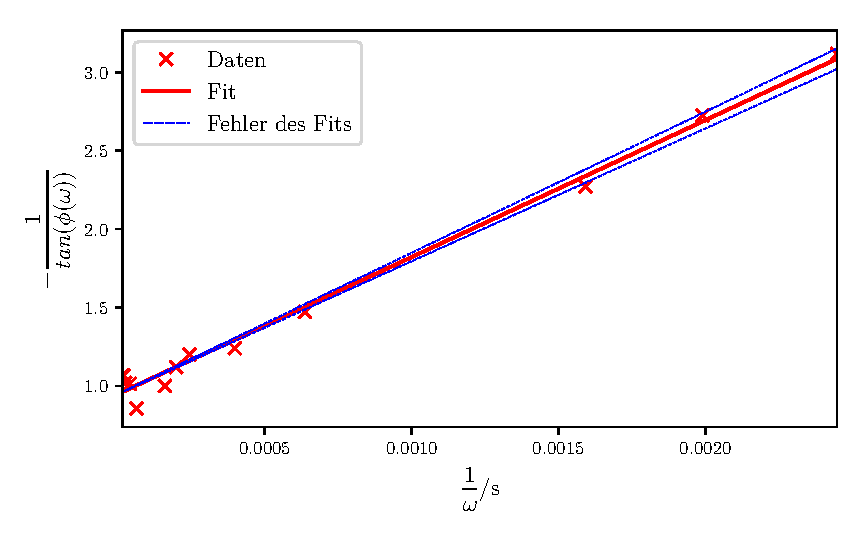
\includegraphics[width=13cm, height=9cm]{build/plotc.pdf}
  \caption{Auftragung des negativen Kehrwerts des Tangens der Phase, die sich durch die negative Division der 
  zeitlichen Phasenverschiebung durch die Periodendauer multipliziert mit $\pi$ ergibt gegen den Kehrwert der 
  Kreisfrequenz. Dargestellt werden die Daten und der dazugehörige Fit. Die Skala ist logarithmiert.}
  \label{fig:plotc}
\end{figure}

\noindent Mittels \eqref{eqn: RC} und \eqref{eqn: fehler} berechnet sich das Inverse der Zeitkonstante zu
$\frac{1}{RC} = \SI[per-mode=fraction]{873.015 \pm 26.684}{\per\second}$.

\subsection{Abhängigkeit der Relativamplitude von der Phasenverschiebung}
Die Werte, die zur Bestimmung der Abhängigkeit der Relativamplitude $\frac{A(\omega)}{U_{0}}$ von der
Phasenverschiebung $\phi$ nötig sind, befinden sich in Tabelle \ref{tabd}.
\begin{table}\caption{Die Phasenverschiebung gegen die Amplitude der Spannung $U_{C}$ geteilt durch die maximale Spannung $U_{0}}
\label{tabd}
\centering
\sisetup{round-mode = places, round-precision=5, round-integer-to-decimal=true}
\begin{tabular}{S[]S[]} 
\toprule
{$\phi/ \si{\radian}$} & {$\frac{A(\omega)}{U_{0}}$}\\
\midrule
-0.31038935417467156 & 0.9146537842190016\\
-0.3518583772020568 & 0.8631239935587762\\
-0.4146902302738527 & 0.7858293075684379\\
-0.5969026041820606 & 0.4347826086956522\\
-0.6785840131753953 & 0.286634460547504\\
-0.6942919764433444 & 0.1819645732689211\\
-0.728849495632832 & 0.14814814814814814\\
-0.7853981633974483 & 0.14814814814814814\\
-0.8639379797371932 & 0.04830917874396135\\
-0.7791149780902686 & 0.03027375201288245\\
-0.7759733854366789 & 0.01884057971014493\\
-0.7539822368615503 & 0.015619967793880838\\
-0.7539822368615503 & 0.012399355877616747\\
\bottomrule
\end{tabular}\end{table}
Um die verschiedenen errechneten Werte für die Zeitkonstante $RC$ vergleichen
zu können, wird für die in \ref{sec: a}, \ref{sec: b} und \ref{sec: c} berechneten Werte in den folgenden Abbildungen
\ref{fig: plotd1}, \ref{fig: plotd2} und \ref{fig: plotd3} die Relativamplitude $\frac{A(\omega)}{U_{0}}$ als Radius
und die Phase $\phi$ als Winkel dargestellt. Die rote Linie entspricht den berechneten Werten 
$\frac{A(\omega)}{U_{0}}$, die durch Einsetzen von $\phi$ in die Formel \eqref{eqn: A1} bestimmt werden. Die grüne Linie entspricht der 
Theoriekurve, welche durch die Formel \eqref{eqn: phi} mit den Werten für $RC$ bestimmt wird.
\begin{figure}
  \centering
  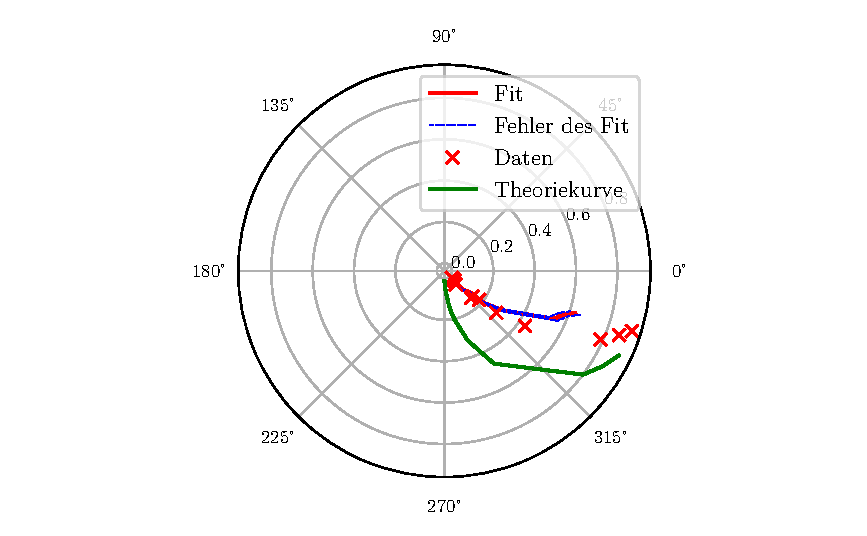
\includegraphics[width=12cm, height=7cm]{build/plotd1.pdf}
  \caption{Abhängigkeit der Relativamplitude in Abhängigkeit von der Phase für die in \ref{sec: a} 
  berechnete Zeitkonstante in einem Polarkoordinatensystem dargestellt. Es sind Daten, ein Fit, der Fehler
  des Fits und die Theoriekurve eingezeichnet.}
  \label{fig: plotd1}
\end{figure}

\begin{figure}
  \centering
  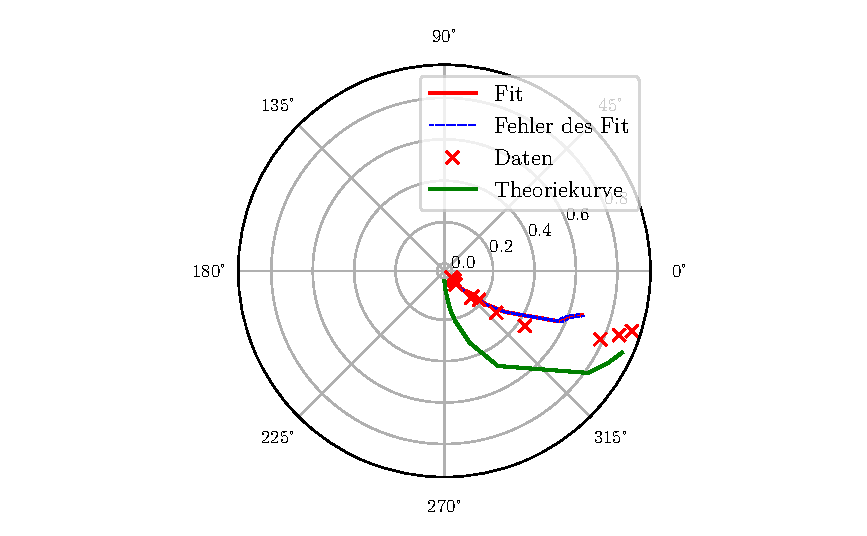
\includegraphics[width=12cm, height=7cm]{build/plotd2.pdf}
  \caption{Abhängigkeit der Relativamplitude in Abhängigkeit von der Phase für die in \ref{sec: b} 
  berechnete Zeitkonstante in einem Polarkoordinatensystem dargestellt. Es sind Daten, ein Fit, der Fehler
  des Fits und die Theoriekurve eingezeichnet.}
  \label{fig: plotd2}
\end{figure}

\begin{figure}
  \centering
  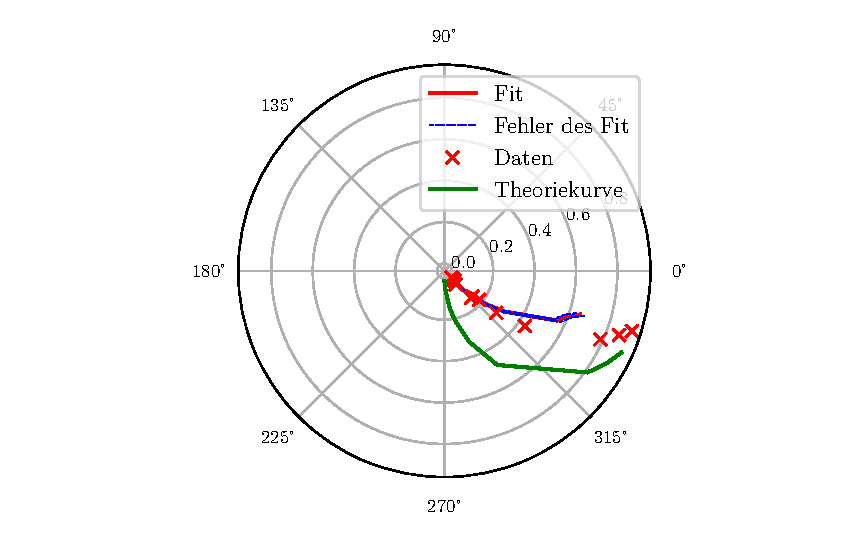
\includegraphics[width=12cm, height=7cm]{build/plotd3.pdf}
  \caption{Abhängigkeit der Relativamplitude in Abhängigkeit von der Phase für die in \ref{sec: c} 
  berechnete Zeitkonstante in einem Polarkoordinatensystem dargestellt. Es sind Daten, ein Fit, der Fehler
  des Fits und die Theoriekurve eingezeichnet.}
  \label{fig: plotd3}
\end{figure}

\subsection{Spannung als Integrator}
%Integrator Bilder
Die folgenden Abbildungen zeigen die integrierte, sowie die zu integrierende Spannung.
Dabei wird eine Sinusspannung angelegt. Die Kondensatorspannung wird dadurch zu einem Cosinus. Die Dreiecksspannung wird zu einer Funktion integriert, die einem Sinus ähnelt. Die Rechteckspannung integriert sich zur Dreiecksspannung. \newline \newline \newline %Noch was?
\begin{figure}
  \centering
  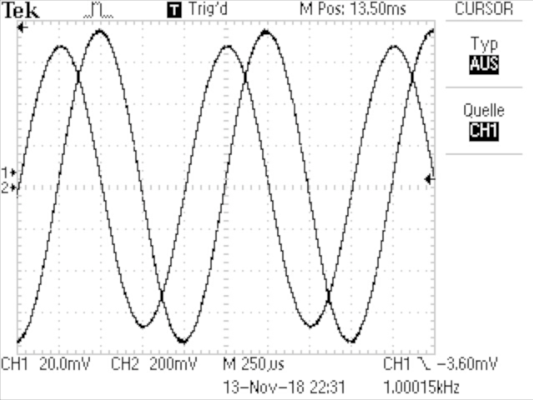
\includegraphics[width=9cm, height=6cm]{build/integrator1.pdf}
  \caption{Aufnahme des Bildschirms des Oszillokops bei eingestellter Sinusspannung.}
  \label{fig: sinus}
\end{figure}

\begin{figure}
  \centering
  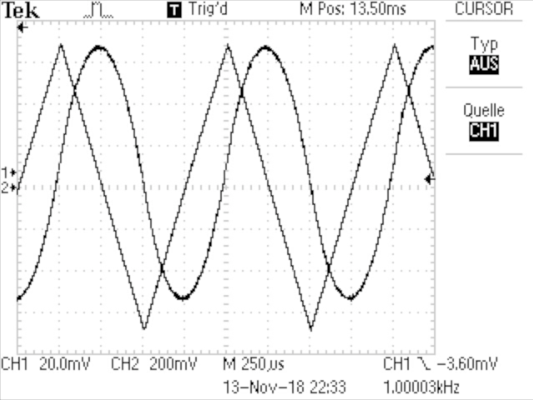
\includegraphics[width=9cm, height=6cm]{build/integrator2.pdf}
  \caption{Aufnahme des Bildschirms des Oszillokops bei eingestellter Dreiecksspannung.}
  \label{fig: dreieck}
\end{figure}

\begin{figure}
  \centering
  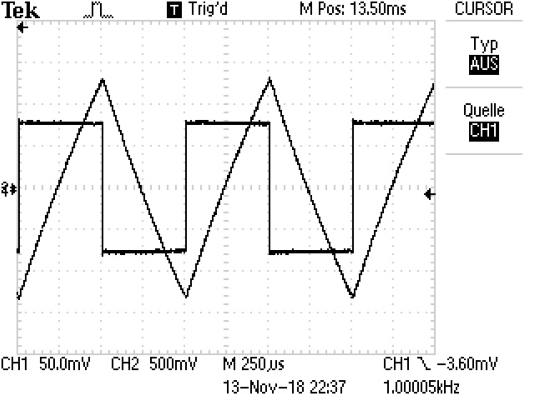
\includegraphics[width=9cm, height=6cm]{build/integrator3.pdf}
  \caption{Aufnahme des Bildschirms des Oszillokops bei eingestellter Rechteckspannung.}
  \label{fig: rechteck}
\end{figure}



